% Kopfzeile beim Kapitelanfang:
\fancypagestyle{plain}{
%Kopfzeile links bzw. innen
\fancyhead[L]{\Large Vorlesung 4 (24.10.2013)}
%Kopfzeile rechts bzw. außen
\fancyhead[R]{}}
%Kopfzeile links bzw. innen
\fancyhead[L]{\Large Vorlesung 4 (24.10.2013)}
%Kopfzeile rechts bzw. außen
\fancyhead[R]{}
% **************************************************
\phantomsection
\addcontentsline{toc}{section}{Allgemeines Assoziativ- und Kommunitativgesetz}
\section*{Allgemeines Assoziativ- und Kommunitativgesetz}
$x_1+x_2+\hdots+x_n := (\hdots((x_1+x_2)+x_3)+\hdots)$\\
Wiederholte Anwendung des A- und K-Gesetzes zeigt: Das Eregbnis ist unabhängig von Klammerung (also Klammern weglassen!) und Reihefolge.\\
Das gilt auch für Produkte.

\section*{Potenzen}
Sei $x \in K$.\\
Für $n \in \N$ setze $x^n := \underbrace{x \cdot x \cdot \hdots \cdot x}_{n \text{ Faktoren}}$ mit $x^0=1$\\
Falls $x \neq 0$ setze $x^{-1} := (x^{-1})^n$\\
Damit: $x^{-n} = (x^n)^{-1}$\\
Regeln für $x,y \in K$ und $n,m \in \N_0$ seien:
\items{
\item $x^n x^m = x^{n+m}$
\item $x^n y^n = (xy)^n$
\item $(x^n)^m = x^{nm}$
}
Falls $x,y \neq 0$ gelten diese Regeln auch für alle $n,m \in \Z$.

\subsection*{Beispiele}
$\R$ und $\Q$ sind Körper mit den üblichen Operationen.\\
$\Z$ ist kein Körper, denn nur $+1$ und $-1$ haben multiplikative Inverse.

\subsection*{Beispiel eines endlichen Körpers}\label{BspEndlKoerper}
$\F_2=\{0,1\}$ mit Operationen wie folgt:\nl
\begin{tabular}{c|c|c}
$+$ & $0$ & $1$ \\ 
\hline 
$0$ & $0$ & $1$\\
$1$ & $1$ & $0$
\end{tabular}\hspace{5em}
\begin{tabular}{c|c|c}
$\cdot$ & $0$ & $1$ \\ 
\hline 
$0$ & $0$ & $0$\\
$1$ & $0$ & $1$
\end{tabular}\nl
Nachweis des Axioms: direktes Nachprüfen.\\
In $\F_2$ gilt: $1+1=0$

\newpage

\phantomsection
\addcontentsline{toc}{section}{Definition: Anordnungsaxiome}
\section*{Definition: Anordnungsaxiome}\label{Anordnungsaxiome}
$\R$ enthält eine Teilmenge von Elementen, die als positiv ausgezeichnet sind (Schreibweise: $x>0$).
\begin{enumerate}[label=(A\arabic*)]
\item Jedes $x \in \R$ genügt genau eine der Beziehungen $x>0$, $x=0$, $-x>0$ (Trichotomie)
\item $x>0 \wedge y>0 \Rightarrow x+y>0, x \cdot y > 0$
\end{enumerate}

\subsection*{Beziehungen}
$x>y \Leftrightarrow x-y>0$\\
$x<y \Leftrightarrow y>x$\\
$x \ge y \Leftrightarrow x>y \vee x=y$\\
$x \le y \Leftrightarrow y \ge x$

\section{Folgerungen}\label{3.4}
\en{
\item $x<0 \Leftrightarrow -x>0$
\item $\forall x,y \in \R$ gilt genau eine der Beziehungen $x>y, x=y, x<y$
\item $x<y \wedge y<z \Rightarrow x<z$ (Transitivität)
\item $x<y, z \in \R \Rightarrow x+z<y+z$ 
\item $x<y \Leftrightarrow -y < -x$
\item $x<y \wedge a < b \Rightarrow x+a < y+b$
\item $x<y \wedge a > 0 \Rightarrow ax < ay$ (i)\\
$x<y \wedge a < 0 \Rightarrow ax > ay$ (ii)
\item $0 \le x < y, 0 \le a < b \Rightarrow ax < by$\\
Folgerung (mit $a=x, b=y$): $0 \le x < y \Rightarrow x^2 < y^2 \Rightarrow x^n < y^n$ ($\forall n \in \N$)
\item $x \neq 0 \Rightarrow x^2 > 0$, insbesondere $1=1 \cdot 1 > 0$
}

\subsection*{Beweise}
\en{
\item $x<0 \Leftrightarrow 0>x \Leftrightarrow 0-x=-x>0$
\item aus Trichotomie für $x-y$
\item $z-x=(z-y)+(y-x)>0$
\item bilde Differenz
\item bilde Differenz
\item $(y+b)-(x+a)=\underbrace{(y-x)}_{>0} + \underbrace{(b-a)}_{>0} > 0$
\item (i) $ay-ax=\underbrace{a}_{>0} \underbrace{(y-x)}_{>0} > 0$\\
(ii) $a<0 \Rightarrow -a>0$ analog
\item In der Übung
\item Falls $x>0$: $\Rightarrow x^2>0$\\
Falls $x<0$: $\Rightarrow [\text{7.(ii) mit }y=0, a=x]\,x^2>0$
}

\newpage

\section{Definition: Angeordnete Körper}\label{3.5}
Ein Körper $K$, in dem eine Teilmenge von Elementen als positiv ausgezeichnet ist ($x>0$), so dass die Axiome (A1) und (A2) gelten, heißt \underline{angeordneter Körper}.\\
Die Folgerungen 3.5 gelten in jedem angeordneten Körper.\nl
$\R$ und $\Q$ sind angeordnete Körper.\\
$\F_2$ ist kein angeordneter Körper, denn in $\F_2$ gilt: $1+1=0$\\
Annahme: $\F_2$ wäre angeordnet. $\Rightarrow 1>0 \Rightarrow 1+1 > 0$ \wspruch

\section{Bernoulli-Ungleichung}\label{3.6}
Sei $x \in \R$, $x>-1$ und $n \in \N_0$.\\
Dann ist $(1+x)^n \ge 1+nx$.

\subsection*{Beweis mit vollständiger Induktion}
\en{
\item Induktionsanfang: $n=0$\\
$(1+x)^0 = 1 = 1+0 \cdot x$ \ok
\item Induktionsvoraussetzung: Die Bernoulli-Ungleichung gelte für ein beliebiges, festes $n$.
\item Induktionsschluss: $n \rightarrow n+1$\\
$(1+x)^{n+1} = \underbrace{(1+x)}_{>0} \cdot \underbrace{(1+x)^n}_{>=1 \text{ nach IV}} \ge (1+x) \cdot (1+nx)$\\
$=1+(n+1)x+nx^2 \ge 1+(n+1)x$ \ok
}
\qed

\section{Definition: Betrag}\label{3.7}
Sei $x \in \R$.\\
$|x| := \left\{
\begin{array}{l l}
x & \quad \text{falls } x \ge 0\\
-x & \quad \text{falls } x<0
\end{array} \right.$\\
Insbesondere: $|x| \ge 0$ und $|-x|=|x|$\\
Anschaulich: $|x|$ ist der Abstand von $x$ und $-x$ zu $0$.\\
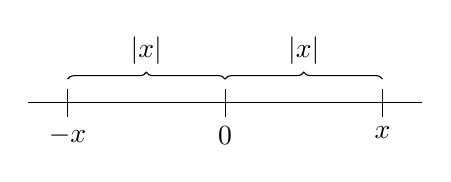
\begin{tikzpicture}[decoration=brace]
% Die Grundlinie:
\draw(0,0)--(5,0);
\foreach \x/\xtext in {0.5/$-x$,2.5/$0$,4.5/$x$}
  \draw(\x,5pt)--(\x,-5pt) node[below] {\xtext};
\draw[decorate, yshift=2ex]  (0.5,0) -- node[above=0.4ex] {$|x|$}  (2.5,0);
\draw[decorate, yshift=2ex]  (2.5,0) -- node[above=0.4ex] {$|x|$}  (4.5,0);
\end{tikzpicture}

\newpage

\section{Satz: Regeln für Beträge}\label{3.8}
\en{
\item $|x| \ge 0$ wohei $|x|=0 \Leftrightarrow x=0$
\item $|xy| = |x| \cdot |y|$ (Multiplikativität)
\item $\left| \frac{x}{y} \right| = \frac{|x|}{|y|}$ falls $y \neq 0$
\item $|x+y| \le |x|+|y|$ (Dreiecksungleichung)
}

\subsection*{Beweise}
\en{
\item Klar aus Definition \ok
\item $|xy| \in \{\pm xy\}, |x| \cdot |y| \in \{\pm xy\}$\\
Beide sind $\ge 0 \Rightarrow$ Gleichheit \ok
\item $x=\frac{x}{y} \cdot y \Rightarrow |x|=\left|\frac{x}{y}\right| \cdot \underbrace{|y|}_{\neq 0} \Rightarrow$ Behauptung \ok
\item $\pm x\le|x|, \pm y\le|y| \Rightarrow \pm(x+y)\le|x|+|y| \Rightarrow$ Behauptung \ok
}
\qed

\phantomsection
\addcontentsline{toc}{section}{Intervalle}
\section*{Intervalle}\label{Intervalle}
Seien $a,b \in \R$ mit $a \le b$.
\en{
\item Abgeschlossenes Intervall: $[a,b] := \{x \in \R : a \le x \le b\}$\\
\begin{tikzpicture}[decoration=brace]
\draw[->](0,0)--(5,0);
\foreach \x/\xtext in {0.5/$a$,2.5/$x$,4.5/$b$}
  \draw(\x,-5pt) node[below] {\xtext};
\draw(0.5,0pt) node{[};
\draw(4.5,0pt) node{]};
\end{tikzpicture}
\item Offenes Intervall: $(a,b) := \{x \in \R : a < x < b\}$\\
\begin{tikzpicture}[decoration=brace]
\draw[->](0,0)--(5,0);
\foreach \x/\xtext in {0.5/$a$,2.5/$x$,4.5/$b$}
  \draw(\x,-5pt) node[below] {\xtext};
\draw(0.5,0pt) node{(};
\draw(4.5,0pt) node{)};
\end{tikzpicture}
\item Halboffene Intervalle: $[a,b) := \{x \in \R : a \le x < b\}$ und $(a,b] := \{x \in \R : a < x \le b\}$\\
\begin{tikzpicture}[decoration=brace]
\draw[->](0,0)--(5,0);
\foreach \x/\xtext in {0.5/$a$,2.5/$x$,4.5/$b$}
  \draw(\x,-5pt) node[below] {\xtext};
\draw(0.5,0pt) node{[};
\draw(4.5,0pt) node{)};
\end{tikzpicture}
\begin{tikzpicture}[decoration=brace]
\draw[->](0,0)--(5,0);
\foreach \x/\xtext in {0.5/$a$,2.5/$x$,4.5/$b$}
  \draw(\x,-5pt) node[below] {\xtext};
\draw(0.5,0pt) node{(};
\draw(4.5,0pt) node{]};
\end{tikzpicture}
\item Uneigentliche Intervalle: $[a,\infty) := \{x \in \R : x \ge a\}$ und $(\infty,a] := \{x \in \R : x \le a\}$\\
\begin{tikzpicture}[decoration=brace]
\draw[->](0,0)--(5,0);
\foreach \x/\xtext in {0.5/$a$}
  \draw(\x,-5pt) node[below] {\xtext};
\draw(0.5,0pt) node{[};
\end{tikzpicture}
\begin{tikzpicture}[decoration=brace]
\draw[->](0,0)--(5,0);
\foreach \x/\xtext in {4.5/$a$}
  \draw(\x,-5pt) node[below] {\xtext};
\draw(4.5,0pt) node{]};
\end{tikzpicture}
}

\newpage

\section{Definition: Vollständigkeitsaxiom}\label{3.9}
\emph{In eckigen Klammern stehendes bezieht sich auf ``nach unten beschränkt''}\nl
$M \subseteq \R$ heißt \underline{nach oben [unten] beschränkt} $\Leftrightarrow \exists s \in \R : x \le s \forall x \in M$ [$x \ge s \forall x \in M$]\\
Das $s$ ist dann die \underline{obere [untere] Schranke von $M$}.\\
Eine obere [untere] Schranke, die in $M$ liegt, ist das \underline{Maximum [Minimum] von $M$}.\\
$M$ heißt \underline{beschränkt} $\Leftrightarrow M$ ist nach oben \underline{und} unten beschränkt.\\
\begin{tikzpicture}[decoration=brace]
\draw[->](0,0)--(5,0);
\foreach \x/\xtext in {0.75/$t$,2.5/$M$,4.25/$s$}
  \draw(\x,-5pt) node[below] {\xtext};
\draw(1.5,0pt) node {$|$};
\draw(3.5,0pt) node {$|$};
\end{tikzpicture}

\subsection*{Beispiele}
\en{
\item $M=[0,1] \Rightarrow M$ ist beschränkt.\\
Jedes $s \ge 1$ ist obere Schranke und jedes $t \le 0$ ist untere Schranke von $M$.\\
$1$ ist Maximum, $0$ ist Minimum von $M$ ($1=\text{max }M$ und $0=\text{min }M$).
\item $M=[0,1)$\\
$M$ hat kein Maximum, denn es gibt kein $m \in [0,1)$, welches obere Schranke des Intervalls ist.\\
Es gibt immer größere Zahlen, die sich auch im Intervall befinden. ($m < \underbrace{\frac{1}{2}(m+1)}_{\in [0,1)} < 1$)
\item Das Intervall, das zur linken Seite geöffnet ist, hat kein Minimum (analog).
}